\documentclass[../main.tex]{subfiles} 
\begin{document}
\chapter{Low-Level softwarebeveiliging}
\section{Introductie}
Een \emph{implementation-level software vulnerability} is een fout in een programma die door een aanvaller kan worden misbruikt.
In dit hoofdstuk hebben we het concreet over \emph{memory corruption vulnerabilies}.
Deze zwakheden zijn enkel relevant voor onveilige talen.
Dat zijn programmeertalen die niet controleren of programma's het geheugen correct gebruiken.
Hieronder staat een voorbeeld in ANSI c in listing \ref{l:intro}. Omdat er nergens de lengte van de input argumenten wordt nagekeken kan men in geheugen schrijven waar dat niet zou mogen.
Op die manier kan er arbitraire code worden uitgevoerd (een \emph{code injection attack}).
 
\lstinputlisting[style=cstyle, label=l:intro]{\codeSrc/intro_example.c}

\subsection{Achtergrond informatie}
Er kan op verschillende manieren geheugen gealloceerd worden in C:
\begin{description}
	\item[Automatisch] via locale variablen in functies.	
	\item[Statisch] via globale variablen.	
	\item[Dynamisch] via \lstinline[style=cstyle]{void *malloc(size_t size);} en \lstinline[style=cstyle]{new}.
\end{description}
De programmeur is verantwoordelijk voor dit geheugenbeheer van het alloceren tot het de-alloceren.
Figuur \ref{f:mem_lay} geeft de \emph{process memory layout} weer van een programma.
Hierbij groeit de heap naar boven (hogere adressen) en de stack naar onder (lagere adressen).
Indien de voorbeeld code \ref{l:intro} wordt ge\"exploiteerd bevind de geinjecteerde code zich in de Stack.
\begin{figure}
\centering
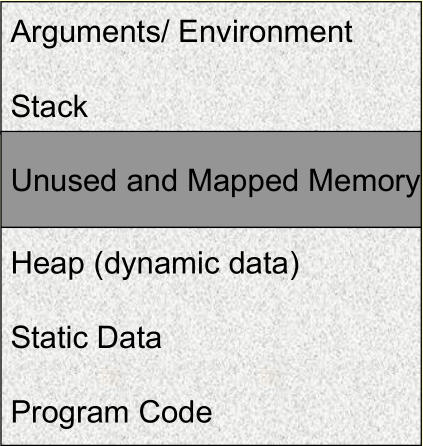
\includegraphics{\imageSrc/memory_layout.png}
\caption{Typische geheugen layout met bovenaan \textbf{hoge} adressen. De stack groeit van hoge naar lage adressen en de heap van lage naar hoge adressen.}
\label{f:mem_lay}
\end{figure}

Memory management in C is zeer fout-gevoelig typische bugs zijn o.a.:
\begin{itemize}
		\item Writing past the bound of array (zoals in listing \ref{l:intro})
		\item Dangling pointers (pointers die niet naar een geldig object wijzen.)
		\item Double freeing (Twee keer \lstinline[style=cstyle]{free()} aanroepen zodat nog gebruikt geheughen als ongebruikt wordt gemarkeert).
		\item Memory leaks (Stukken geheugen zijn niet correct vrijgegeven.)
\end{itemize}
Om effici\"entie redenen worden deze fouten in C niet at run time gededecteert.

Om onveilige code aan te vallen moet een aanvaller hetvolgende doen:
\begin{itemize}
		\item Een bug vinden die memory safety breekt.
				\begin{itemize}
						\item Buffer overflow
						\item Dereference van dangling pointer
						\item Gebruik van onveilige API functie. Die ofwel een buffer overflowt (e.g. \lstinline[style=cstyle]{strcpy()} ofwel intrinsiek onveilig geimplementeerd is in assembly (e.g. \lstinline[style=cstyle]{printf()}
				\end{itemize}
		\item Een interessante geheugen plaats vinden om te overschrijven.
				\begin{itemize}
								\item Code adressen/pointers: Return address, Function pointer in Virtual function table, Programma specifieke fuction pointers
								\item Pointers waar de aanvaller kan controleren wat er wordt geschreven als die dereferenced raakt (= Indirect pointer overwrite): redirect de pointer naar een andere interessante locatie en schrijf dan daar een zekere waarde.
				\end{itemize}
		\item Aanvals code in het geheugen van het process plaatsen.
\end{itemize}

\section{Aanvals voorbeelden}
\subsection{Stack-based buffer overflow}
De stack is een geheugen gebied dat wordt gebruikt om functie oproepen en returns at run time te beheren.
Per oproep wordt er een \emph{activation record} of \emph{stack frame} op de stack gepusht. Daarin zitten parameters, return address, lokale variablen, \ldots
Het is eenvoudig in te zien dat als er nu een lokale variable kan worden overflowt dat er interessante geheugen plaatsen ter beschikking komen.

In de onderstaande figuren leggen we een typisch Stack Based Buffer Overflow uit. Opgelet ook hier weer veronderstellen we dat bovenaan hoge addressen staan en dus overflowt een buffer naar boven.
In figuur \ref{f:stackBO1} tonen we een normale (niet aangevallen) stack waarbij het laatste stackframe dat van functie f0 is. De instructiepointer (IP) aan het begin van f0 staat en de (Saved) Frame Pointer ((S)FP) en Stack Pointer (SP) staan aangeduid.
\begin{figure}
\centering
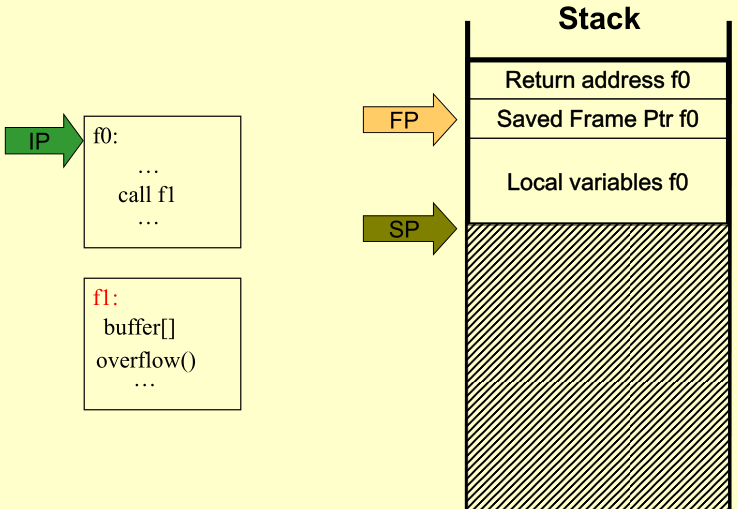
\includegraphics[scale=0.7]{\imageSrc/stackBO1.png}
\caption{Stack layout als de laatst opgeroepen functie f0 is.}
\label{f:stackBO1}
\end{figure}

Vervolgens in figuur \ref{f:stackBO2} wordt functie f1 opgeroepen. Een nieuw stackframe wordt op de stack gepusht. Let hierop dat in dit frame het return address nu wijst naar code net onder de call naar f1. De SFP wijst naar het frame van f0 en er daarachter plaats is voorzien voor de lokale variable \lstinline[style=cstyle]{buffer[]}. De stackpointer wijst natuurlijk net voorbij het frame van f1.
\begin{figure}
\centering
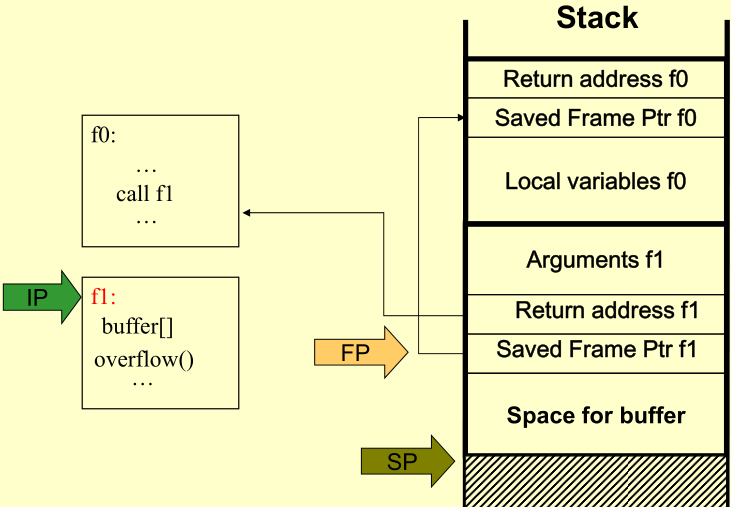
\includegraphics[scale=0.7]{\imageSrc/stackBO2.png}
\caption{Stack layout na call van functie f1.}
\label{f:stackBO1}
\end{figure}

In deze figuur wordt de overflow aangeduid. Als er geen bounds check gebeurdt kan de buffer blijven groeien en zo eerst de SFP, en dan het return address overschrijven. Door nu in het buffer uitvoerbarde code te steken en het return address naar die code te doen verwijzen kan er alles met het programma worden gedaan.
\begin{figure}
\centering
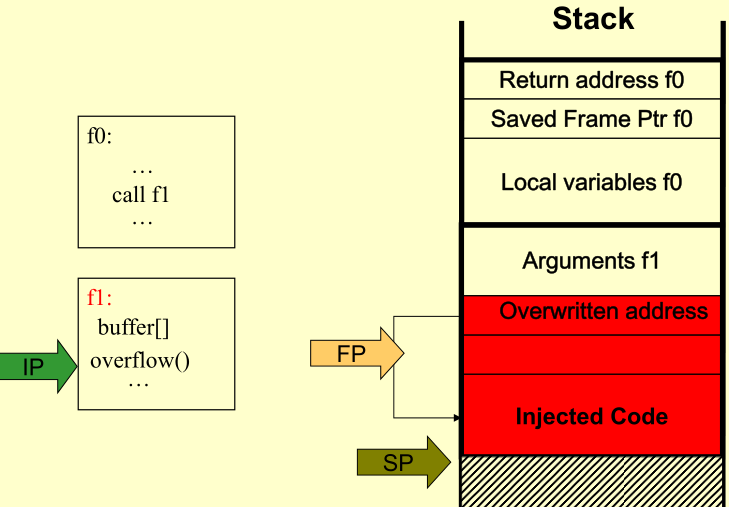
\includegraphics[scale=0.7]{\imageSrc/stackBO3.png}
\caption{Stack layout na buffer overflow attack op de lokale variable buffer in functie f1.}
\label{f:stackBO3}
\end{figure}
Het voorbeeld dat we in de introductie zagen (zie listing \ref{l:intro}) is een goed voorbeeld van een programma kwetsbaar voor een buffer overflow attack.

Code die vaak wordt gebruikt om te injecteren is het starten van een nieuwe shell.
Om dit te doen wordt er zogenaamde shellcode gebruikt.
Dit is een string van hexadecimale codes die dan worden geinterpreteerd als programma code.
Hieronder vind u een voorbeeld die op Linux systemen met een intel x86 architectuur kan gebruikt worden om de \emph{sh} shell te starten.

\begin{blockquote}
	"\textbackslash xeb\textbackslash x1f\textbackslash x5e\textbackslash x89\textbackslash x76\textbackslash x08\textbackslash x31\textbackslash xc0\textbackslash x88\textbackslash x46\textbackslash x07\textbackslash x89\textbackslash x46\textbackslash x0c\textbackslash xb0\textbackslash x0b \textbackslash x89\textbackslash xf3\textbackslash x8d\textbackslash x4e \\\textbackslash x08\textbackslash x8d\textbackslash x56\textbackslash x0c\textbackslash xcd \textbackslash x80\textbackslash x31\textbackslash xdb\textbackslash x89\textbackslash xd8\textbackslash x40\textbackslash xcd\textbackslash x80\textbackslash xe8\textbackslash xdc\textbackslash xff\textbackslash xff\textbackslash xffbin/sh"
\end{blockquote}

Om een stack based buffer overflow werkend te krijgen zijn er heel veel details waar de aanvaller rekening mee moet houden: O.a. 

\subsection{Heap-based buffer overflow}
Soms bevatten programmas enkel een overflowbare buffer die op de heap gealloceerd is.
Bijvoorbeeld globaal gedeclareerde structuren.
Aangezien die zich niet op de stack bevinden is er geen return address dicht bij.
Wel zijn er andere manieren om toch een succesvolle code injection attack te doen waarvan we er hier twee bekijken: overwriting function pointer en overwriting heap metadata.
\subsubsection{Overwriting function pointer}
In listing \ref{l:heapBO} staat een programma dat kwetsbaar is voor een heap based buffer overflow door middel van een function pointer te overschrijven. 
\lstinputlisting[style=cstyle, label=l:heapBO]{\codeSrc/heapBO.c}

Figuur \ref{f:heapBO1} toont hoe de vulnerability wordt uitgebuit.
In (a) zien we de opeenvolgende adressen van de struct en de waardes die ze initieel krijgen toegekent.
In (b) zien we hoe er een overflow kan worden gerealiseerd die cmp overschrijft.

Let hierbij op het feit dat de waardes in Little Endian worden opgeslagen.
Dit betekend dat de eerste byte van een geheugenlocatie de meest rechtse positie krijgt.
We kunnen dit makkelijk zien door het einde van het voorbeeld (b)te bekijken. De laatste drie characters van de string zijn ``sdf''.
We weten dat ``s'' overeenkomt met het hexadecimale ``73'', d met ``64'' en f met ``66''.

Als we nu naar de geheugen locatie van cmp (\emph{0x00353078}) kijken dan vinden we daar \emph{0x00666473}. 
Tabel
\begin{table}
\centering 
\begin{tabular}{l|cccc|}
		Geheugen plaats (hex) & 0x0035307b & 0x0035307a & 0x00353079 & 0x00353078 \\ \hline
		Geheugen waarde (hex) & 00 & 66 & 64 & 73 \\ \hline
		Character (string representatie) & n/a & f & d & s \\ \hline   
\end{tabular}
\end{table}

\begin{figure}
\centering
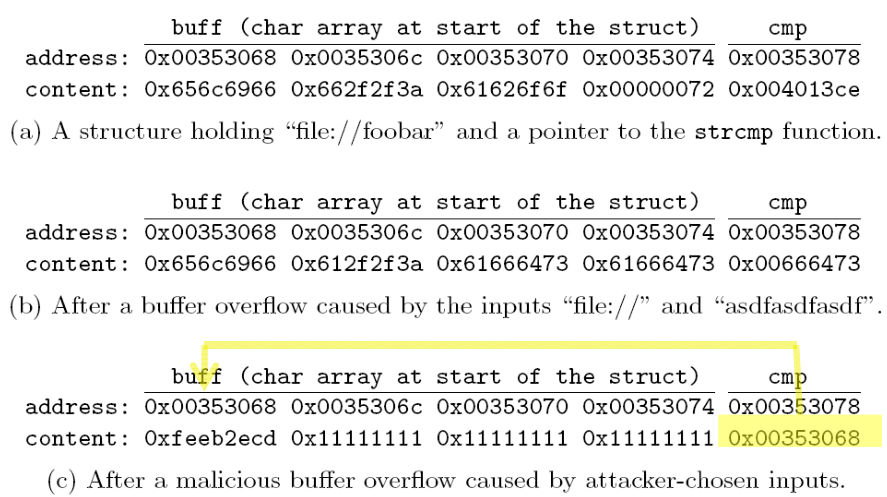
\includegraphics[scale=0.7]{\imageSrc/heapBO1.png}
\caption{Stack layout na buffer overflow attack op de lokale variable buffer in functie f1.}
\label{f:heapBO1}
\end{figure}

\subsubsection{Overwriting heap metadata}
De heap wordt gebruikt om dynamisch gealloceerde data op te slaam.
Met functies zoals \lstinline[style=cstyle]{malloc()} worden er dynamisch geheugenblokken gealloceerd en gedealloceerd met \lstinline[style=cstyle]{free()}.
De meest memory allocation libraries onthouden metadata voor of achter gebruikte blokken.
Een gevolg daarvan is dat buffer overruns op de heap deze management informatie kunnen overschrijven.
Dit maakt een \emph{indirect pointer overwrite} aanval mogelijk. 

Om de aanval te begrijpen kijken we eerst naar hoe de heap er uit ziet in het normale geval.
In figuur \ref{f:heapBO2} vinden we hoe een gebruikt blok en een leeg blok eruit zien.
De lege blokken worden onthouden door ze als dubbel gelinkte lijst te gebruiken.
Achteraan elk blok wordt een backward pointer, forward pointer en wat andere informatie (groote bvb) bijgehouden.
Als een blok gebruikt wordt dan wordt het uit de lijst gehaald door de backward pointer twaalf plaatsen verder te schrijven dan naar waar de forward pointer wijst (en omgekeerd voor de forward pointer).

\begin{figure}
\centering
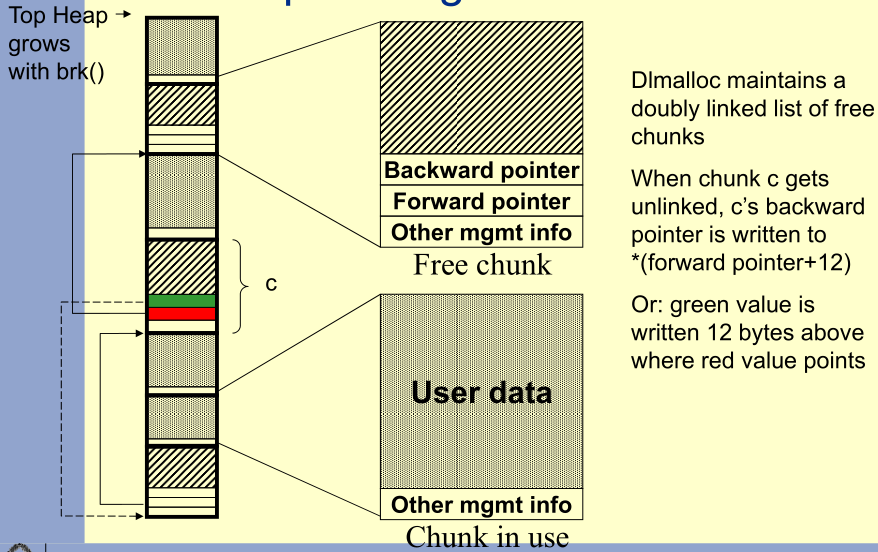
\includegraphics[scale=0.6]{\imageSrc/heapBO2.png}
\caption{Normaal geval in de heap als het lege blok c wordt gebruikt en dus unlinked wordt van de double linked list met vrije blokken.}
\label{f:heapBO2}
\end{figure}

Het idee is nu om dit feit uit te buiten door het unlink mechanisme te gebruiken om het return address van een functie op de stack te vervangen.
In figure \ref{f:heapBO3} wordt er in blok d een buffer geoverflowt zodat de forward en backward pointer van c kunnen overschreven worden.
Concreet gebeurdt dat door de backward pointer (groen) te doen wijzen naar in de buffer waar de geinjecteerde code staat. 
De forward pointer van c moet dan wijzen naar twaalf plaatsen \emph{onder} (er wordt immers bij het unlinken twaalf plaatsen hoger geschreven) het return address (RA) van een functie.
Het eigenlijke resultaat is dat te bezichtigen in \ref{f:heapBO4}.
Van zodra blok c wordt gebruikt zal de aanval opgezet zijn.
Het return address van een zekere functie zal dan immers wijzen naar de geinjecteerde code. 
Van zodra die functie dan returnt zal bijvoorbeeld de shell code worden uitgevoerd.

\begin{figure}
\centering
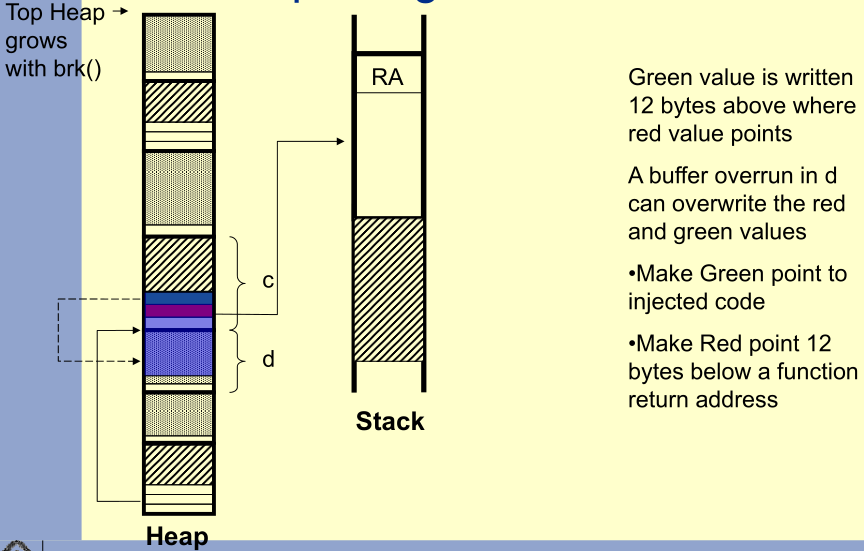
\includegraphics[scale=0.6]{\imageSrc/heapBO3.png}
\caption{Buffer overflow op de heap in actie. Een buffer in blok d wordt overflowt (naar boven in deze figuur) tot in het lege blok c.}
\label{f:heapBO3}
\end{figure}

\begin{figure}
\centering
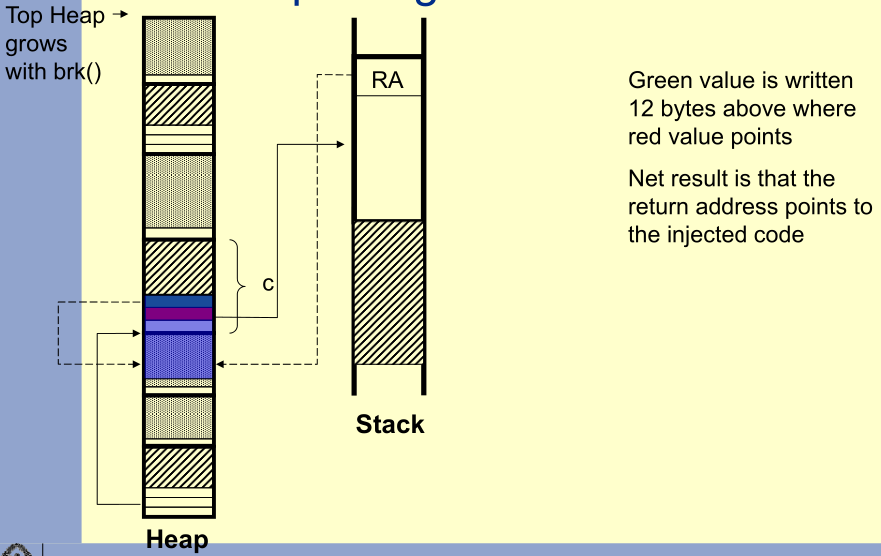
\includegraphics[scale=0.6]{\imageSrc/heapBO4.png}
\caption{Resultaat van een indirect pointer overwrite door middel van een buffer overflow op de heap.}
\label{f:heapBO4}
\end{figure}

Deze aanval wordt ook wel een indirect pointer overwrite genoemd.
De aanval is breed inzetbaar in verschillende situaties.
Een programma is kwetsbaar voor zo'n aanval als het drie elementen bevat:
\begin{itemize}
		\item Een bug die toelaat een pointer te overschrijven.
		\item Die pointer wordt later gedereferenced om te schrijven.
		\item En de waarde die geschreven wordt kan worden gecontroleerd door de attacker.
\end{itemize}


\begin{figure}
\centering
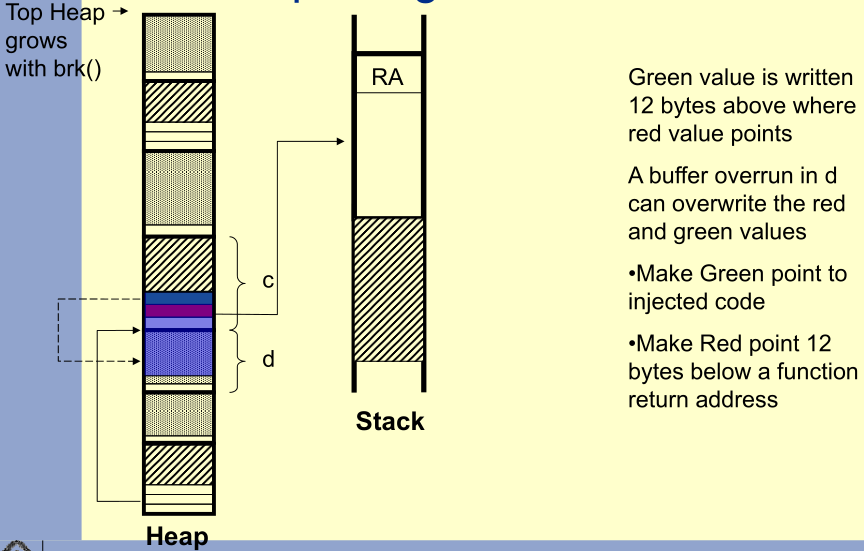
\includegraphics[scale=0.6]{\imageSrc/heapBO3.png}
\caption{Buffer overflow op de heap in actie. Een buffer in blok d wordt overflowt (naar boven in deze figuur) tot in het lege blok c.}
\label{f:heapBO3}
\end{figure}

\begin{figure}
\centering
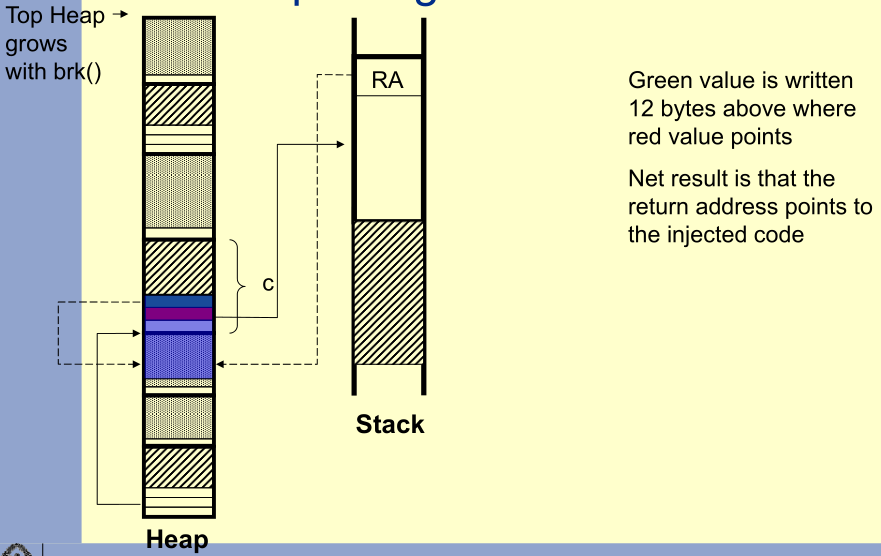
\includegraphics[scale=0.6]{\imageSrc/heapBO4.png}
\caption{}
\label{f:heapBO4}
\end{figure}
\subsection{Return-to-libc attacks}
Tot nu toe hebben we altijd rechtstreek code kunnen injecteren in een buffer.
Dit is niet altijd mogelijk aangezien er een countermeasures kunnen genomen worden om dit te voorkomen.
Wel bestaan er dan Indirect code injection attacks die het programma sturen door het manipuleren van de stack.
Dit maakt het mogelijk om stukken code uit te voeren die al in het geheugen zitten en meestal is er zo'n code beschikbaar bvb. libc.

Figuren \ref{f:libc1} en \ref{f:libc2} tonen hoe het returnen uit een functie de stack beinvloed.
\begin{figure}
\centering
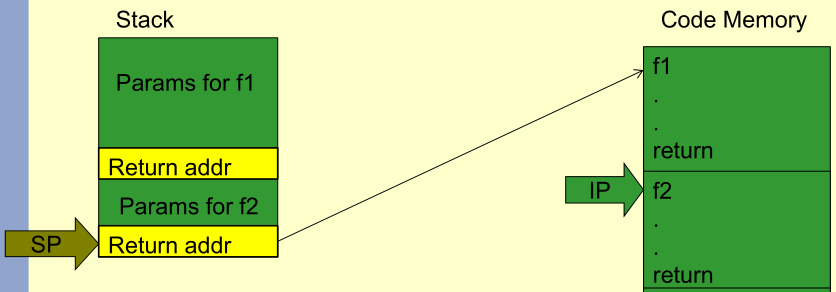
\includegraphics[scale=0.8]{\imageSrc/libc1.png}
\caption{Stack als functie f2 gaat returnen. De Stack Pointer (SP) en Instruction Pointer (IP) zijn aangeduid.}
\label{f:libc1}
\end{figure}

\begin{figure}
\centering
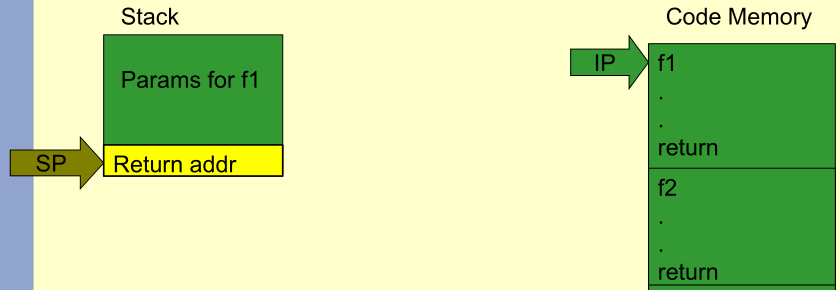
\includegraphics[scale=0.8]{\imageSrc/libc2.png}
\caption{Stack als functie f2 gereturned heeft en enkel nog het f1 stackframe op de stack staat.}
\label{f:libc2}
\end{figure}

Aangezien we de werking van de stack doorhebben kunnen we dat gebruiken om de stack na te bootsen.
Een nagebootste stack kan gewoon in een buffer wordten opgeslagen.
De fake stack kan bijvoorbeeld een functie aanroepen die een shell start of het mogelijk maakt om andere code rechtstreeks te injecteren.
Vervoglens moeten we de SP doen wijzen naar de fake stack net voor de return instructie van de actieve functie wordt uitgevoerd.

\textit{Meer uitleg volgt mogelijk nog}

\lstinputlisting[style=cstyle, label=l:libc]{\codeSrc/libc.c}

\subsection{Data-only attacks}
Dit soort aanvallen bestaat erin enkel de data van een programma te veranderen.
Afhankelijk van die data kan dit tot interessante exploits leiden.
We bekijken er hier twee: Unix password attack en overwriting the environment table.
\subsubsection{Unix password attack}
In figuur \ref{f:UnixPA} staat een voorbeeld van een onveilig passwoord controlerend programma.
In een oude versie van unix werd dit gebruikt maar dit is eenvoudig te omzeilen.
Als er immers een passwoord wordt ingegeven dat bestaat uit \emph{pw || hash(pw)} en het pw is lang genoeg dan overflowt het passwoord in de hash.
Bijgevolg zal er altijd toegang worden verschaft.

\begin{figure}
\centering
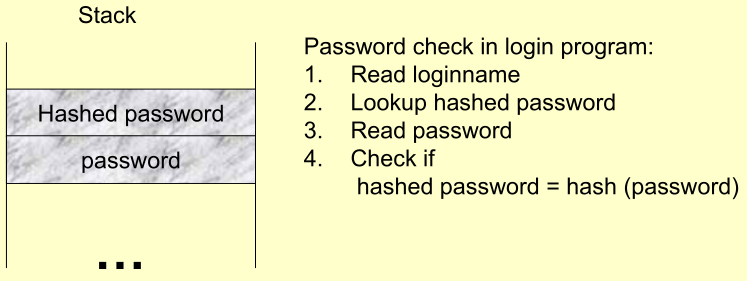
\includegraphics[scale=0.8]{\imageSrc/unixPA.png}
\caption{Voorbeeld van onveilig password checking programma.}
\label{f:unixPA}
\end{figure}

\subsubsection{Overwriting the environment table}

\section{Verdedigings voorbeelden}
\subsection{Stack canaries}
\subsection{Non-executable data}
\subsection{Control-flow integrity}
\subsection{Layout randomization}
\section{Conclusie}
\end{document}
